\setchapterpreamble[u]{\margintoc}
\chapter{Technology Costs}
\labch{technology_costs}

In this chapter I will go over estimating the technology costs, per unit of energy installed and produced, for the low carbon options and their necessary ancillaries\sidenote[][-2mm]{We will come back to that, but there is debate on the "low" part of "low carbon" for some of the technologies}. 

\begin{kaobox}[frametitle=Low Carbon Energies]
As a reminder, those low carbon energies are:

\begin{itemize}
	\item Wind
	\item Solar
	\item Water
	\item Nuclear
	\item Biomass
\end{itemize}

Storage is the necessary ancillary for 100\% non-controllable renewable scenarios.

\end{kaobox}


Technology costs can be difficult to account for fully. For example, renewable energy, due to their decentralized nature and their high output variability, require significant, and often considered separately, transmission grid upgrades. As we will discuss, storage becomes prevalent in 100\% Renewable scenarios. And finally, the costs vary a lot by location, even within a single country, and over short periods of time.

\section{Nuclear}

Nuclear costs data varies a lot by country, depending on the workforce, the red tape, the NIMBYsm (Not In My Backyard) delays, the political will, and other considerations. Some projects are utter failures, while other seem quite successful. Hinkley Point C Power Plant, in the UK, is predicted to be four times more expensive than the identical Taishan Power Plant in China\sidenote[][-2mm]{It is an important point that we will have to consider later on. This demonstrates less a nuclear problem and more a loss of competence at building large ambitious projects}.

The prices are obtained for advanced nuclear reactors as well as small modular reactors from the EIA. 

We see that the capital cost is estimated at around \$6,100 per kW for both systems. The cost of dismantling a reactor is estimated to be between \$600 and \$1,500 per kW\sidenote[][-2mm]{In France, EDF is estimating the cost at \$350 per kW. Maybe, maybe not. I would not bet on it. At the same time, the UK is estimating the cost at up to \$3,200 per kW. Again, maybe, maybe not. And again, I would not bet on it}. Historically, hazardous waste industrial facilities dismantlement in different industries has been shown to cost around 10\% of the capital cost, which validates our estimated range further despite the lack of actual data points. A value of \$1,000 per kW of dismantlement will be used. Keep in mind that this cost is not as big as one would think in the grand scheme of transition, and that even tripling it would not impact the conclusions we will get at.

The lifetime of a nuclear plant can be taken as 60 years. It typically ranges from 40 to 80 years, with 40 years being very pessimistic, and 80 years requiring significant upgrades over the years.


\section{Gas with Carbon Capture}

\blindtext


\section{Solar}

We use the research from the National Renewable Energy Laboratory (NREL) for the cost of photovoltaic storage data. They also compute the cost of a photovoltaic and storage combined installation, but we will for now ignore those results, as we will want to account for those separately at a grid level (Feldman, 2021).


\begin{figure}[hb]
	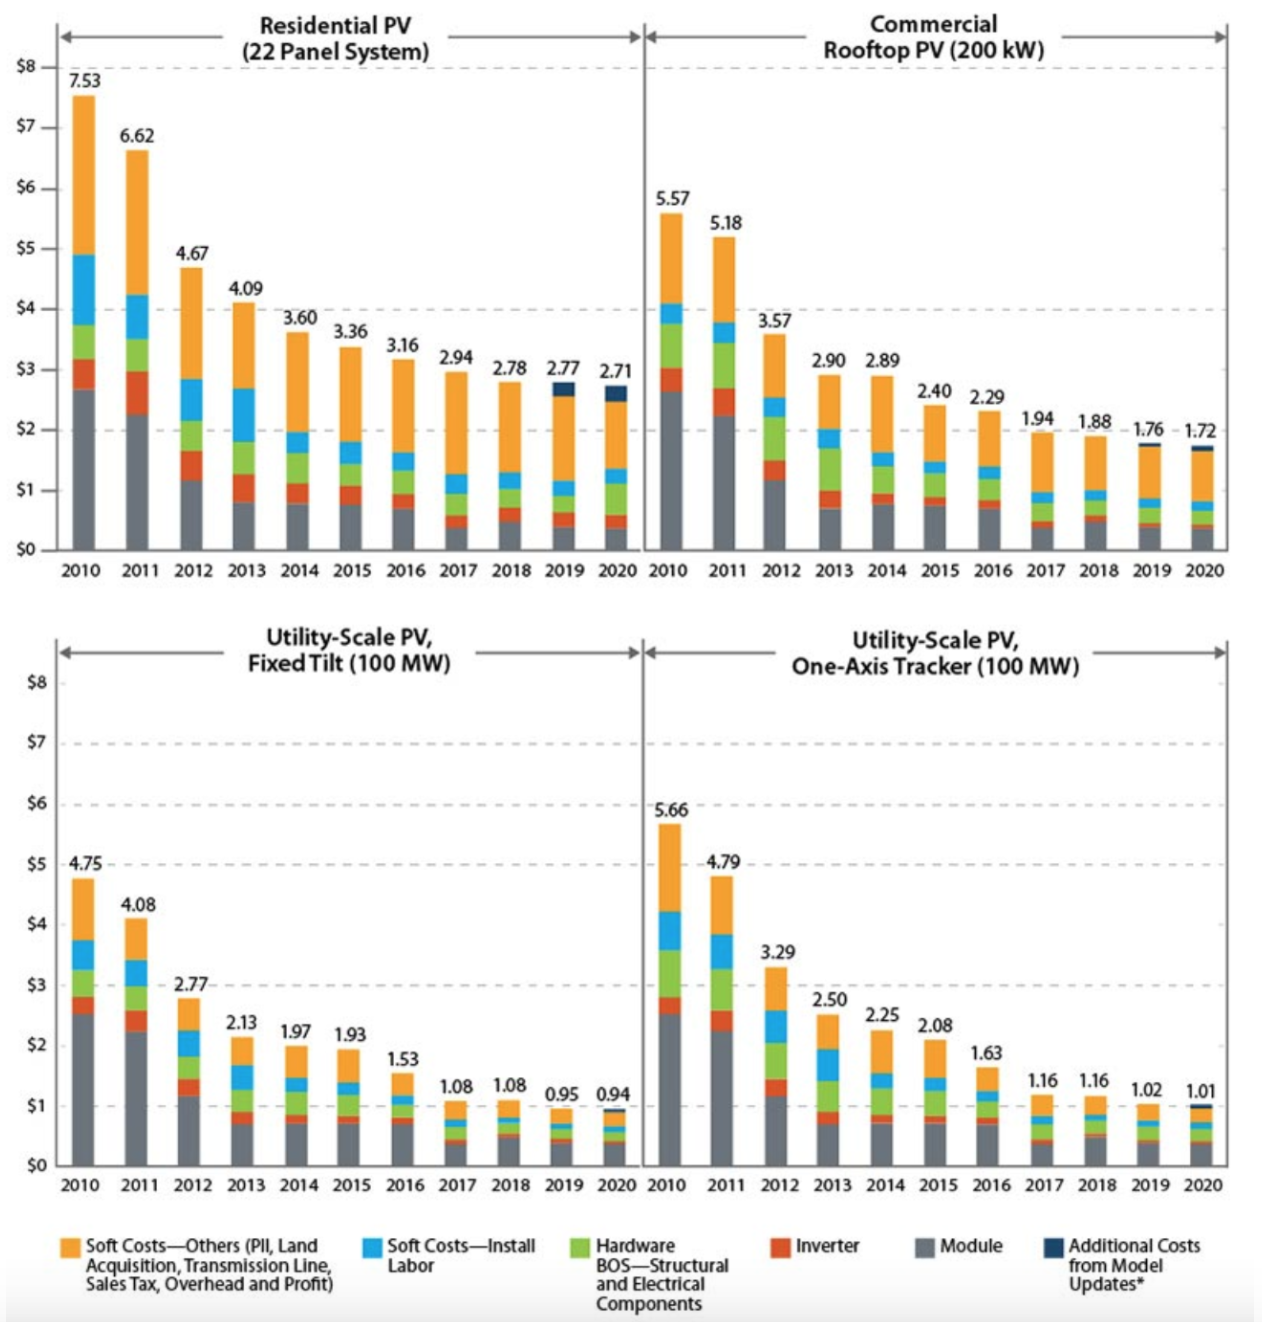
\includegraphics[width=1.0\textwidth]{solar_costs_evolution}
	\caption[Evolution of photovoltaic costs over the last decade, for several system sizes (\$/W)]{Evolution of photovoltaic costs over the last decade, for several system sizes (\$/W).}
	\labfig{solar_costs_evolution}
\end{figure}

What \vreffig{solar_costs_evolution} shows is that while the cost of installing a solar panel went down significantly over the past decades, most of the easy optimization has been done and the rate of price reduction is quickly decreasing, showing an exponential trend\sidenote[][-2mm]{In my experience, this is often glossed over in the media by simply saying that the prices for solar keep going down. Technically true, I will admit that, but nuance is always important}.

We can note that utility scale is separated into two main categories, a fixed tilt (your panel does not move) and a one-axis tracker (your panel follows the sun). The gain in load factor of the latter category is often offset by the cost difference. In this study, we will focus on the fixed tilt, while keeping in mind that a few optimizations could be done, without changing the overall conclusions.

So, what we can conclude from \vreffig{solar_costs_evolution} is that, indeed, the costs of solar energy have plummeted even in the last decade. However, we are reaching a limit that will be difficult to break through.

Consequently, in this calculation, we will assume that the current price of solar (remember, it is location dependent) is \$940 per kW, and that we can only realistically expect few gains over the next decades.


\begin{marginfigure}[-2mm]
	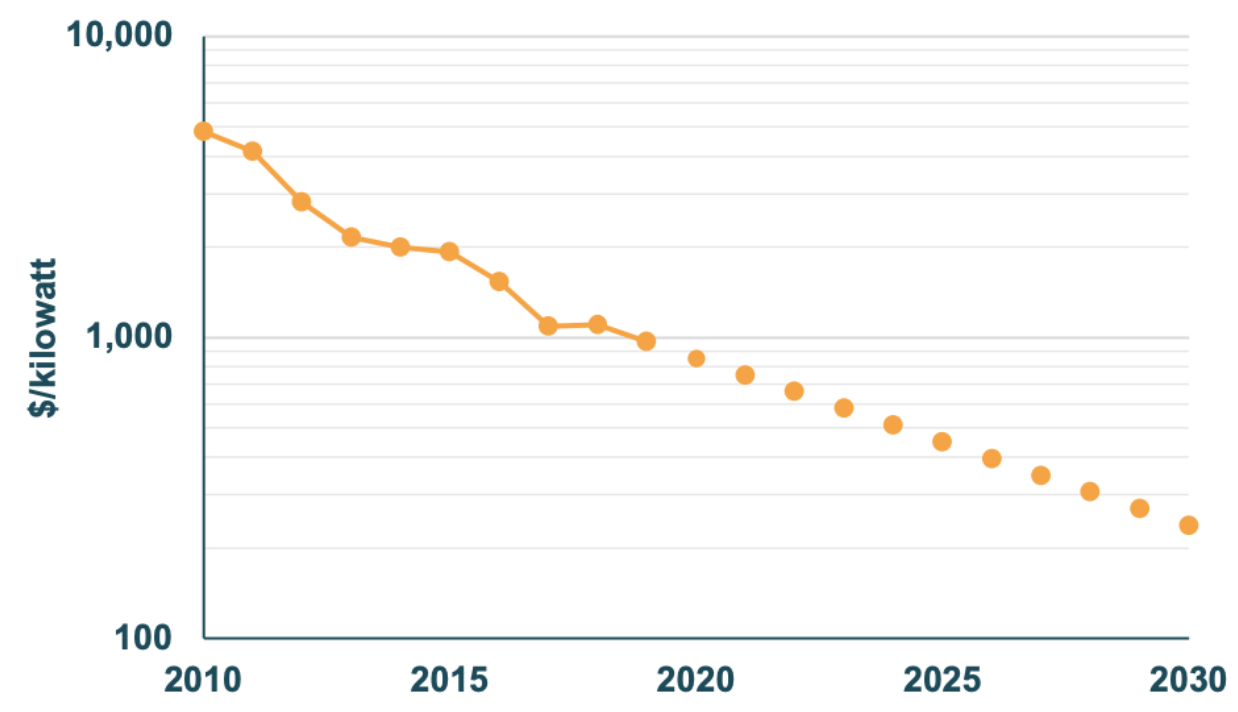
\includegraphics{dorr_optimistic_solar_costs}
	\caption[An interestingly optimistic view of the future... Solar energy manufacturing, installation and maintenance will be absolutely free before the end of the century according to some. A good reminder to be careful with your extrapolations, and the use of logarithmic scales]{An interestingly optimistic view of the future...\\ Solar energy manufacturing, installation and maintenance will be absolutely free before the end of the century according to some. A good reminder to be careful with your extrapolations, and the use of logarithmic scales.}
	\labfig{dorr_optimistic_solar_costs}
\end{marginfigure}

The lifetime of a solar installation is around 25 years. Of course, it does not fail exactly at 25 years. But degradation rates are a non negligible issues, so even if it lasts a bit longer, the gains are not enormous. We can tweak this value to test the sensitivity later on.


\section{Wind}

The wind costs have not been falling as sharply as solar in recent years. As can be seen in an NREL report on 2019 costs, onshore wind turbines will set you back around \$1,436 per kW, and offshore wind turbines around \$4,077 per kW (Stehly, 2020). It is indeed a lot more complicated to build and maintain an offshore turbine, due to the harsh ocean environment. There is a clear upside to that though, as the wind is more constant and drastically increases the load factor.

The lifetime of a wind turbine is around 25 years, give or take a few, and a little less for an offshore wind turbine, due to the harsher conditions.



\begin{figure}[hb]
	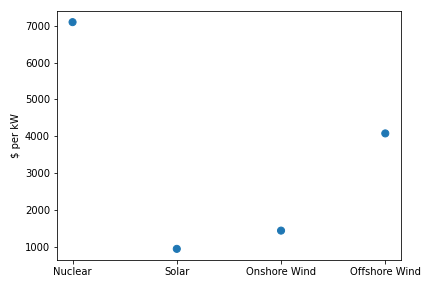
\includegraphics[width=1.0\textwidth]{technology_costs}
	\caption[2020 capital costs estimate to install various technologies]{2020 capital costs estimate to install various technologies.}
	\labfig{technology_costs}
\end{figure}


\vreffig{technology_costs} shows a damning picture for nuclear doesn't it? It is simply too expensive, several times the cost of solar and onshore wind, and even offshore wind project would be way cheaper. This is what most people, from media to politics, base their financial estimates on. And it is technically true.

But, and you knew a "but" was coming, this is misleading. Why is it misleading? Two main reasons:


\begin{itemize}
	\item Lifetime
	\item Controllable energy
\end{itemize}

A nuclear power plant has a much longer lifetime than a renewable plant\sidenote[][-2mm]{Except hydroelectricity!}. Even though, per kW, your cost is way cheaper, you do need to install several times as many kW over a long enough period of time.

On top of this, nuclear energy is a controllable energy. You turn down the dial, you have less power. You turn it up, you have more power. Solar and Wind are non controllable energy sources. We do not decide when the sun will shine or when the wind will blow. Interestingly, with the sun, we have a pretty good idea of the production times, as we know for a fact that no energy will be output at night. But cloud cover varies (fast) and we are simply not able to model it currently, and probably never will. Wind has a higher load factor, as seen previously, but the variations are quite important and unpredictable.


\begin{kaobox}[frametitle=Controllable versus Non Controllable]
A controllable energy is an energy that you control. You can decide how much power you will output and (relatively) quickly adapt to the demand consumption quick changes.

A non controllable energy is an energy that you do not control. If it's sunny, you have some, and the amount you get depends on how sunny it is, not on a button you turn. If it's not sunny, you are out of luck and must wait until the sun (or the wind) comes back to turn your TV back on. 
\end{kaobox}


\marginnote[-1cm]{There is one thing that I would like to point out, and here is as good a place as any. The low (and falling) cost of manufacturing of solar panels and wind turbines is, in part, due to easy and cheap energy sources for industrial activities, provided by fossil fuels. While I am not quantifying that value, it is not that far-fetched to see that removing that access may impact the manufacturing costs negatively, especially during a transition phase.}

What this means is that one cannot simply compare the cost of nuclear energy with the cost of solar or wind energies, as the metrics are not measuring the same things. It is the same units, \$ per kW, but the respective kW are two very different things depending on their ability to be controlled.



\begin{kaobox}[frametitle=Levelized Cost Of Electricity]
You will sometimes see the term LCOE, which stands for Levelized Cost of Electricity. What this metric does is account for time in the comparison, so that the lifetime discrepancy is corrected for.

A lot of people takes the LCOE at face value, and argue that it is the value to consider. In the current energy mix, this is correct. However, the controllability difference is still not considered, and at high enough penetration of renewable (and any 100\% renewable scenario), this does not hold true anymore from a purely physical point of view. You can install as many solar panels as you want, when it's night time, you get zero power, which you cannot afford in modern society.
\end{kaobox}


\section{Storage}

Now, we have seen the cost of installing solar and wind energy. Is that enough? Well, if we consider a 100\% Renewable scenario, we need a way to efficiently dispatch electricity to cover the varying demand.


As mentioned previously, we are going to make an assumption that I am convinced you will tend to agree with. We do want a cleaner world\sidenote[][-2mm]{We actually need it}, but we still want Netflix, we still want a choice of clothes, we still want our phones, we still want our burgers, we still want to turn on the lights whenever we want to, we still want to be able to take the train or the car to go places,\ldots In short, we still want a world at least similar to the one we are living in today. Sure, we can and will likely have to make some sacrifices and be more aware of what we can do on a day to day basis, be mindful of when to do the laundry or turn on the oven. But comfort is not going away without a fight. Additionally, I personally hope the impoverished of the world\sidenote[][-2mm]{The ones who will be disproportionately affected by climate change, remember\ldots} will have access to a better life and rise to a level of comfort at least somewhat similar to us today, which means access to energy.

So, assuming this, and accounting for a 100\% renewable energy world, it is easy to see that to meet our needs, the means of production will have to become controllable. This is where energy storage comes into play.

We will consider multiple options, from the proven pumped storage stations to the highly hyped battery energy storage system\sidenote[][-2mm]{Often simply called “batteries” or “grid-scale batteries” in the news articles you may have come across}. Pacific Northwest National Laboratories (PNNL) data will be used as reference. Interestingly, they give a value in 2018 as well as an estimated projection up to 2025. In this report, we will consider the more advantageous 2025 values given (Mongird, 2019).

For a battery energy storage system, out of the multiple options available (Sodium-Sulfur, Li-Ion, Lead Acid, Redox Flow, \ldots), the cheapest is selected, that is Li-Ion, at \$1,446  per kW and \$362 per kWh. The lifetime of such batteries is 10 years, maybe 15 years could be doable by 2025.

\begin{kaobox}[frametitle=Energy storage: kW versus kWh]
Recall the energy storage section for the difference between the cost per kW (power capacity, what you can store) and the cost per kWh (energy capacity, what you can get back)
\end{kaobox}


Let’s now look at the more classical options, namely pumped storage stations (PHS) and below-ground compressed air energy storage (CAES). According to the same PNNL report, pumped storage clocks in at a cost of \$2,638 per kW and \$165 per kWh, while compressed air storage is given at around \$1,669 per kW and \$105 per kWh. The lifetime of a pumped storage station has been estimated to be around a century, while a compressed air storage system is given at 25 years.

While compressed air storage is cheaper, the conversion ratio, or in other words the losses incurred by the storage and restitution of the energy is much lower.

Consequently, we will for now consider the best storage technology on the long term, which is the pumped storage hydroelectric solution. It is coincidentally the only one that has really been used at a non-negligible scale and for a long time. We will come back to the other technologies later on.


\section{Grid}

The grid network is very often overlooked. It is now a cost that is folded into an energy source technology, despite the fact that it depends strongly on what energy is being used.

Those costs are extremely difficult to project, especially for a 100\% renewable system for which no data point exists. Studies (IER, 2019) have shown a cost roughly a third of the investment in the production means themselves (solar panels, wind turbines). However, countries currently developing it, such as Germany, have seen an actual cost impact on production of 100\%. In other words, 1 dollar spent on the installed renewable capacity required another dollar invested onto the grid infrastructure.

In this study, we will consider the value above of one-third of the investments made, which correspond to roughly \$500 per kW renewable installed. A sensitivity analysis will also be performed to see the impact of modifying this parameter.

\section{Summary}

\begin{table*}[ht]
\caption[2020 technology costs estimates]{2020 technology costs estimates}
\labtab{technology_costs_estimates}
\begin{tabular}{ c c c c }
	\toprule
	Technology & Capacity Installation & Storage Installation & Grid upgrades \\
	\midrule
	Nuclear & \$7,100 per kW (25y) & Not Applicable & Not Applicable\\
	Solar & \$950 per kW (25y) & \$165 per kWh (100y) & \$500 per kW (50y)\\
	Onshore Wind & \$1,436 per kW (25y) & \$165 per kWh (100y) & \$500 per kW (50y)\\
	Offshore Wind & \$4,077 per kW (25y) & \$165 per kWh (100y) & \$500 per kW (50y)\\
	\bottomrule
\end{tabular}
\end{table*}

